\documentclass{article}
\usepackage{ifthen,graphicx}
\usepackage[top=0.6in, bottom=0.9in, left=0.8in, right=0.8in]{geometry}
%\usepackage[top=1.0in, bottom=1.0in]{geometry}

%\pagestyle{empty}
\newboolean{KEY}
%\setboolean{KEY}{true}   %prints questions and answers
\setboolean{KEY}{false} %prints questions only
\newcommand{\answer}[1]{\ifthenelse{\boolean{KEY}}{#1}{}}
\newcommand{\titleheader}[2]{\ifthenelse{\boolean{KEY}}{#1}{#2}}

\begin{document}
\titleheader{\section*{CS170 SP2019 Quiz 1 Solution}}{\section*{CS170 SP2020 Quiz 1}}

This is a close book, close note quiz. Total points are 10. You have 10 minutes. Good luck. 

\begin{enumerate}

\item What is Unix? What is the relationship of Unix with Linux? [2]

\vspace{1.25in}

\item What are the three parts of Linux? [2]

\vspace{1.25in}


%\item What is Shell in Linux? [1]
%
%\vspace{1in}


\item Briefly explain what do following commands do [6]: 

\begin{enumerate}
\item \texttt{pwd}
\vspace{0.5in}

\item \texttt{man echo}
\vspace{0.5in}

\item \texttt{cd ..}
\vspace{0.5in}

\item \texttt{mkdir newdirectory}
\vspace{0.5in}

\item \texttt{rmdir olddirectory}
\vspace{0.5in}

\item \texttt{ls -l}
\vspace{0.5in}


\end{enumerate}

%\newpage
%\item Briefly explain the two commands in each pair: [6]
%  \begin{enumerate}
%  \item \texttt{pwd}  VS \texttt{passwd} 
%  \vspace{0.3in}
%  \answer{\emph{pwd: current working directory; passwd: change your password}}
%  
%  \item \texttt{rm} VS \texttt{rmdir} 
%  \vspace{0.3in}
%  \answer{\emph{rm: delete a file; rmdir: delete a directory}}
%  
%  \item \texttt{cp} VS \texttt{mv} 
%  \vspace{0.3in}
%  \answer{\emph{cp: copy a file, two files exist; mv: move a file, one file exist}}
%  
%  \item \texttt{cat} VS \texttt{echo} 
%  \vspace{0.3in}
%  \answer{\emph{cat: display the contents of a file to standard output; echo: display a line of text}}
%  
%  \item \texttt{ls} VS \texttt{cd}
%  \vspace{0.3in}
%  \answer{\emph{ls: list files in the current directory; cd: change the current working directory }}
%  
%  \item \texttt{head} VS \texttt{tail} 
%  \vspace{0.3in}
%  \answer{\emph{head: display top 10 lines of the file; tail: display last 10 lines of the file}}
%  
%  \end{enumerate}
%
%\item What Unix command could be used to solve the following question? [3]  
%\begin{enumerate}
%\item Search for a pattern in a file.
%\vspace{0.2in}
%\item Display the content of a file page-wise.
%\vspace{0.2in}
%\item Change the permission on a file or a directory.  
%\vspace{0.2in}
%\item Create a directory.
%\vspace{0.2in}
%\item Get help for a command.
%\vspace{0.2in}  
%\item Get a permission information for a file.
%\vspace{0.2in}
%\end{enumerate}
%
%\answer{\begin{enumerate}
%\item \emph{\texttt{grep}}
%
%\item \emph{\texttt{less}}
%
%\item \emph{\texttt{chmod}}
%
%\item \emph{\texttt{mkdir}}
%
%\item \emph{\texttt{man}}
%
%\item \emph{\texttt{ls -l}}
%
%\end{enumerate}}
%
%
%
%\item What do the following commands do? [6]
%\begin{enumerate}
%\item \texttt{chmod u+x file1.txt}
%\vspace{0.5in}
%\item \texttt{chmod go-w file2.txt} 
%\vspace{0.5in}
%\item \texttt{sort -u file3.txt}  
%\vspace{0.5in}
%\item \texttt{wc -w file4.txt}
%\vspace{0.5in}
%\item \texttt{cd ..} 
%\vspace{0.5in}
%\item \texttt{apropos copy} 
%\vspace{0.5in}
%\end{enumerate}
%
%
%\answer{\begin{enumerate}
%\item \emph{give user or owner execute permission on file1.txt}
%
%\item \emph{remove write permission on file2.txt from group and everyone else}
%
%\item \emph{display file3.txt without any duplicated lines}
%
%\item \emph{count the total number of words in file4.txt}
%
%\item \emph{go to the parent directory}
%
%\item \emph{search copy related command in the system}
%
%\end{enumerate}}
%
%
%\item File system in Unix. Suppose the current working directory is \texttt{mike}.[5]
%\begin{enumerate}
%\item What are the absolute path and relative path for the textfile(in circle) in the following diagram? 
%\begin{center}
%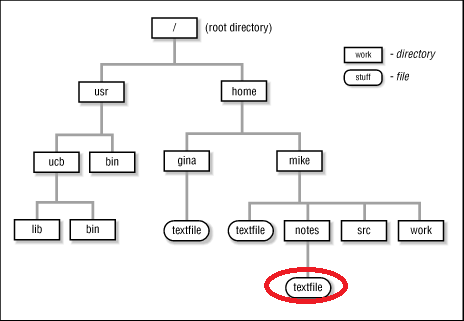
\includegraphics[width=0.45\textwidth]{FilesysExample1}
%\end{center}
%\vspace{1in}
%\item What are the absolute path and relative path for the textfile(in circle) in the following diagram?
%\begin{center}
%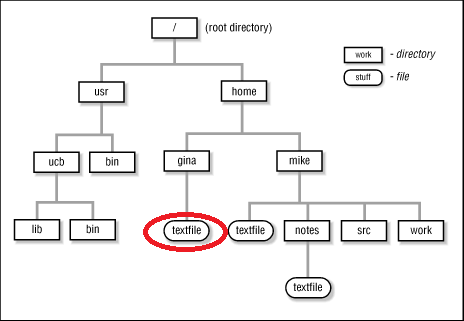
\includegraphics[width=0.45\textwidth]{FilesysExample2}
%\end{center}
%\end{enumerate}
%
%\answer{\begin{enumerate}
%
%\item \emph{absolute path starts with $/$: $/$home$/$mike$/$notes$/$textfile, relative path is notes$/$textfile}
%
%\item \emph{absolute path starts with $/$: $/$home$/$gina$/$textfile, relative path is: ..$/$gina$/$textfile}
%
%
%\end{enumerate}}

\end{enumerate}
\end{document}